\subsection{Aufbau Geiger-Müller-Zählrohrs}
\begin{figure}[h!]
\centering
\includegraphics[scale=0.5]{Grafiken/schema.pdf}
\caption{Der Schematische Aufbau eines Geiger-Müller-Zählrohrs \cite{V703}}
\label{Th1}
\end{figure}
In \cref{Th1} ist der schematische Aufbau eines Geiger-Müller-Zählrohrs zu sehen. Der Mantel wird als Kathodenzylinder bezeichnet und der Stab in der Mitte als Anodendraht. Der zwischen Raum ist mit einem Gasgemisch aus einem Edelgas und wahlweise einem Alkoholgas gefüllt. Die Öffnung ist mit einer Mylarfolie verschlossen und ist aufgrund eines Unterdruckes nach innen gewölbt. Mylar wird dabei als Material gewählt da es dünn genug ist um $\alpha$-Strahlung durchzulassen. Das resultierende elektrische Feld im Hohlraum bei angelegter Spannung $U$ ist gegeben als
\begin{align}
E\left(r\right)=\frac{U}{r\ln\left( r_{\mathrm{k}}/r_{\mathrm{a}} \right)}.
\end{align}

\subsection{Wirkungsweise eines Geiger-Müller-Zählrohrs}
Tritt ein geladenes Teilchen in den Zwischenraum ein, so gibt es seine Energie durch Ironisierung ab. Die Anzahl der Ionisierungsvorgänge ist abhängig von der angelegten Spannung.\\
\begin{figure}[h!]
\centering
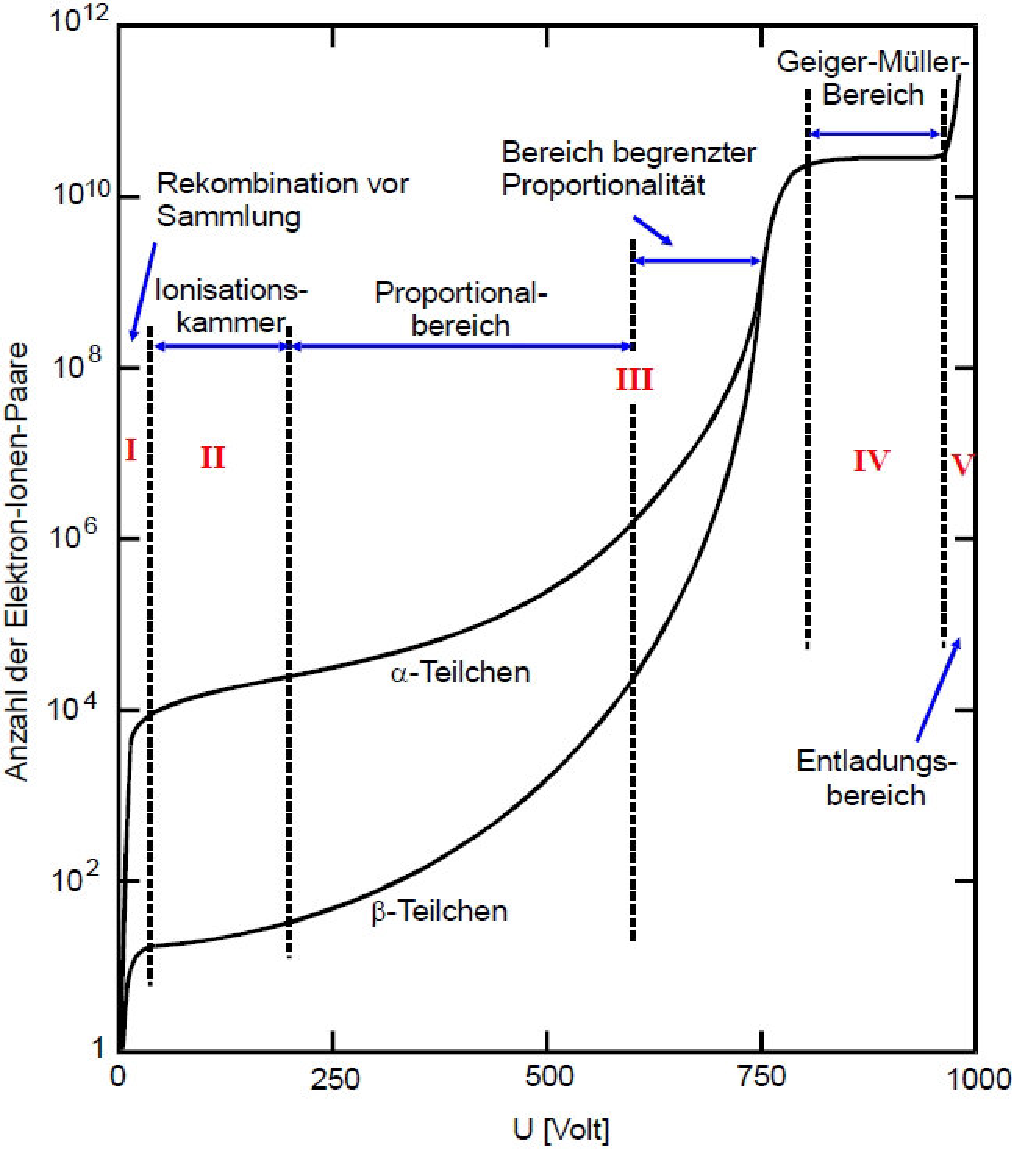
\includegraphics[scale=0.5]{Grafiken/Theorie1.pdf}
\caption{Die Abhängigkeit der erzeugten Elektronen-Ionenpaare zur angelegten\\ Spannung \cite{V703} \label{Th2}}
\end{figure}
Im Spannungsbereich I aus \cref{Th2} erreichen nur eine kleine Anzahl an Elektronen den Anodendraht, weil der Rest durch Rekombination wieder gebunden werden. \\
Bei Bereich II kommen fast alle Elektronen bis zum Draht, dadurch entsteht ein kontinuierlicher Strom, der proportional zur Energie und zur Intensität ist, deshalb kann in diesem Bereich das Geiger-Müller-Zählrohr als Intensitätsmesser verwendet werden, dies wird als \textbf{Ionisationskammer} Bezeichnet.\newpage
Bei höheren Spannungen ist das elektrische Feld in der Nähe des Drahtes so groß, dass die Elektronen beim Zusammenstoß 
mit den Edelgasatomen, weiter ionisieren können. Bei hinreichend hoher Spannung ist es möglich das die freigewordenen 
Elektronen weiter ionisieren können. Dies wird als \textbf{Stoßionisation} bezeichnet und es kommt zu einem 
lawinenartigen Anstieg, der als \textbf{Townsend-Lawine} bezeichnet wird. In diesem Bereich, kann die Zahl der 
einfallenden Ladungen $Q$ in Form von Ladungsimpulsen gemessen werden. Weil die Ladung proportional zur Energie ist, 
kann hier auch die Teilchenenergie gemessen werden. In diesem Bereich entspricht das Geiger-Müller-Zählrohr einem 
\textbf{Proportionalzählrohr}. Dieser Vorgang entspricht Bereich III in \cref{Th2}.\\
Bereich IV ist der Arbeitsbereich des Geiger-Müller-Zählrohrs. Hier ist die Ladung unabhängig von der Primärionisation, 
denn es werden ebenfalls UV-Photonen bei der Ionisation frei gesetzt, die sich im Gegensatz zu den freien Elektronen 
auch senkrecht zur Feldrichtung bewegen können. Sie setzen weitere Elektronen beim Zusammenstoß mit den Edelgasatomen 
frei. Dies hat zur Folge, dass 
die Ladung nur noch von dem Zählrohrvolumen und der angelegten Spannung abhängt. Gemessen wird hier nur noch die 
einfallende Intensität.\\
Im Bereich V wird durch ein einzelnes geladenes Teilchen eine Dauerentladung hervorgerufen. Dies hat zur Folge, dass das Zählrohr schnell kaputt geht.
\subsection{Totzeit und Nachendladungen}
\begin{figure}
\centering
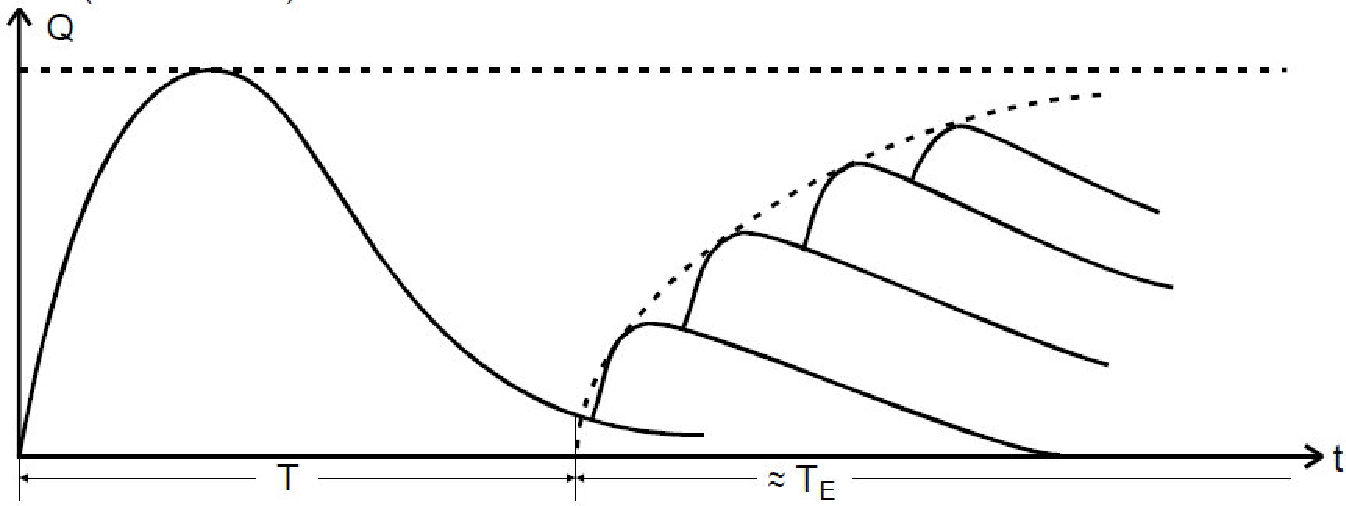
\includegraphics[scale=0.5]{Grafiken/Totzeit.pdf}
\caption{Die qualitative Darstellung de Totzeit und der Erholungszeit \cite{V703}\label{Totzeit}}

\end{figure}
Bei der Ironisierung bleiben positiv geladene Atome übrig, diese setzen für eine Zeit $T$ das elektrische Feld so weit herab, dass Stoßionisation nicht mehr zu lawinenartiger Ionisation führt, da die freien Elektronen wieder rekombinieren (vgl. Bereich I in \cref{Th2}). Das hat zur Folge, dass die in der Zeit eintreffende Strahlung nicht registriert wird, deshalb wird die Zeit \textbf{Totzeit} genannt. Die positiven Ladungen entfernen sich mit der Zeit vom Anodendraht, das bedeutet, dass das elektrische Feld stärker wird, bis es wieder die volle Feldstärke besitzt. Dieser Zeitraum wird \textbf{Erholungszeit} $T_E$ genannt.\\
Es kommt zu \textbf{Nachentladungen}, wenn die positiven Ladungen auf den Kathodenmantel treffen und deren kinetische 
Energie groß genug ist, um weitere Elektronen zu lösen. Diese Elektronen treffen nach der 
\textbf{Laufzeit} $T_L$ auf den Anodendraht. Dies verursacht, dass in der Totzeit etwas gemessen wird und somit 
vortäuscht, dass neue ionisierende Teilchen eintreffen. Dies ist unerwünscht und kann durch das Hinzufügen eines 
Alkohols verhindert werden. Denn sie nehmen reduzieren die kinetische Energie des Edelgases und setzen diese Energie in 
Molekülschwingungen um. Die so abgebremsten Edelgasionen setzen beim Treffen auf den Kathodenmantel keine neuen Elektronen frei.

\subsection{Charakteristik eines Geige-Müller-Zählrohrs}
\begin{figure}[h!]
\centering
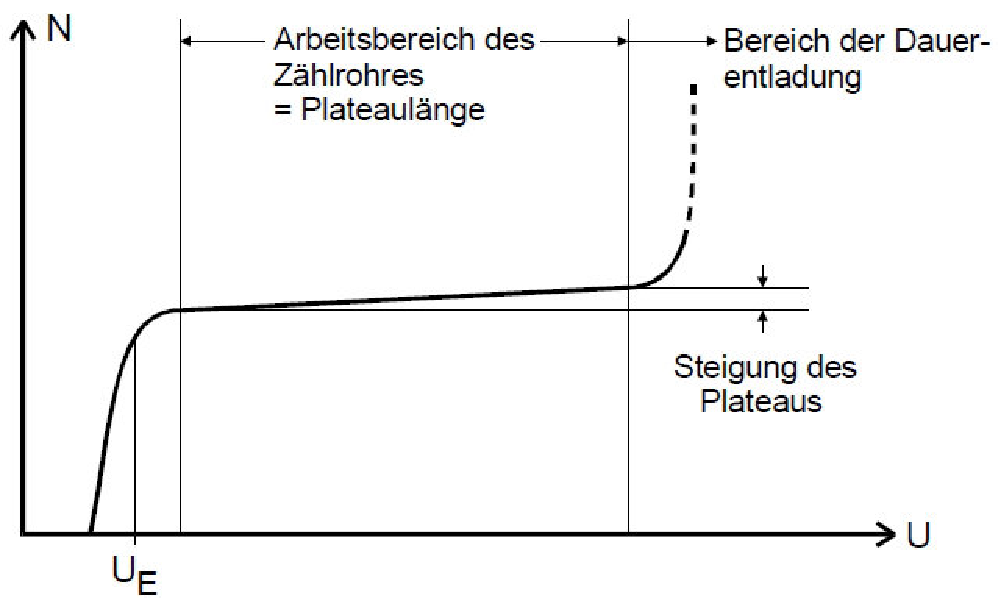
\includegraphics[scale=0.75]{Grafiken/Theorie2.pdf}
\caption{Die qualitative Darstellung, des Plateaus \cite{V703}\label{Th3}}
\end{figure}
Der fast konstante Bereich IV aus  \cref{Th2} wird \textbf{Plateau} genannt. Der leichte Anstieg entsteht durch die Nachentladungen. Ein gutes Geiger-Müller-Zählrohr lässt sich an einer geringeren Steigung des Plateaus und an dessen Länge erkennen.
\subsection{Ansprechvermögen}
Unter dem Begriff \textbf{Ansprechvermögen} wird eine Wahrscheinlichkeit verstanden, mit der ein Teilchen nachgewiesen wird. Durch ihr hohes Ionisationvermögen liegt diese Wahrscheinlichkeit für $\alpha$- und $\beta$-Teilchen bei fast 100$\%$, wenn die Teilchen wirklich in das Zählrohr eindringen. Das kann durch die Mylarfolie gewährleistet werden.\\
Das Ansprechvermögen von Photonen liegt bei ungefähr 1$\%$. Dass bedeutet für $\gamma$-Strahlung, dass nur hohe Intensitäten gemessen werden können. Röntgen-Quanten sind besser zu messen, wenn Xenon als Edelgas verwendet wird.